% Created 2016-08-17 Wed 14:38
\documentclass[tikz]{standalone}

\usepackage[utf8]{inputenc}
\usepackage[T1]{fontenc}
\usepackage{helvet}
\usepackage{../../templates/msc}

\renewcommand{\familydefault}{\sfdefault}

\tikzset{
every picture/.style={
line width=1pt
}}

\usepackage{tikz}
\author{Holger Karl}
\date{\today}
\title{}

\usetikzlibrary{intersections}
\usepackage{xparse}


% snode parameters: 
% 1: number ; 2: state text 
% 3/4: incoming message, 5/6: outgoing ; 7/8: channels
\tikzset{pics/snode/.style 2 args={code={
      \node  (snode#1) {\LARGE P #1};
      \node  (sstate#1) [align=left, below=of snode#1] {\Large State:\\ \Large #2};
      \node (sinA#1) [circle, draw, left=of snode#1] {}; 
      \node (sinB#1) [circle, draw, below=of sinA#1] {}; 
      \node (soutA#1) [circle, draw, right =of snode#1] {}; 
      \node (soutB#1) [circle, draw, below =of soutA#1] {}; 

      \node (srecords#1) [below left=of sstate#1] {}; 
      \coordinate (srecordslow#1) at ([yshift=-1cm]srecords#1);

      \node [draw, fit= (srecords#1) (snode#1) (sstate#1) (sinA#1) (sinB#1) (soutA#1) (soutB#1) (srecordslow#1)] {} ;
}}}

\begin{document}

\newcommand{\nodecanvas}[3]{
\draw (0,0) pic {snode={1}{#1}};

\draw (-6, 4.5) pic  {snode={2}{#2}};

\draw (6, 4.5) pic  {snode={3}{#3}};

\coordinate (lowerLeft) at ([shift={(-1cm, -0.5cm)}]sinB2 |- srecordslow1); 
\coordinate (upperLeft) at ([shift={(-1cm, +1cm)}]sinA2); 

% \node at (lowerLeft) {X}; 
% \node at (upperLeft) {Y}; 

\draw  [->, rounded corners]   (soutB1) -| ++(3.5cm, -1cm) |- (lowerLeft) node (B1B2)  [midway] {} |-  (sinB2); 
\draw [->, rounded corners]   (soutA1) |- node (A1B3)  [near end] {}  (sinB3); 

\draw [->, rounded corners]   (soutB2) -| node (B2A1)  [midway] {} (sinA1); 
\draw [->, rounded corners]   (soutA2) -- node (A2A3)  [midway] {} (sinA3); 

% \coordinate (tmp) at ([yshift=-4.5cm]soutB3 |- sinB1); 
\coordinate (tmp) at ([yshift=-4.5cm] sinB1 -|  soutB2); 
\draw [->, rounded corners]   (soutB3) |- node (B3B1)  [midway] {} (tmp) |-   (sinB1); 
\draw [->, rounded corners]   (soutA3) |- (upperLeft) |- node (A3A2)  [midway] {}  (sinA2); 
}


\NewDocumentCommand\outmess{m m m O{}}{
  \node [draw, fill=gray!20, above right=0.1cm of sout#2#1, #4] {\Large #3}; 
}


\NewDocumentCommand\inmess{m m m O{}}{
  \node [draw, fill=gray!20, above left=0.1cm of sin#2#1, #4] {\Large #3};
}

\NewDocumentCommand\midmess{m m O{}}{
  \node [draw, fill=gray!20, above left=0.1cm of #1, #3] {\Large #2}; 
}


\NewDocumentCommand\records{m m m m m O{}}{
  \node at (srecords#1) [anchor=west, align=left, #6] {
    \large State record: $#2$ \\
     $C_{1#1} = #3$ \\  $C_{2#1} = #4$ \\   $C_{3#1} = #5$};
}


% \begin{tikzpicture}
% \nodecanvas{$S_0$}{$S_1$}{$S_2$}
% \outmess{1}{A}{$M_1$}
% \inmess{2}{B}{$M_2$}
% \midmess{B1B2}{xxx}
% \midmess{A1B3}{xxx}
% \midmess{B2A1}{xxx}
% \midmess{A2A3}{xxx}
% \midmess{B3B1}{xxx}
% \midmess{A3A2}{xxx}
% \end{tikzpicture}

% Step 1: starting point 

\begin{tikzpicture}
  \draw (0,0) pic {snode={1}{$S_1$}};
  
  \node [left=1 cm of sinA1] (inports)  {In ports}; 
  \node [right=1 cm of soutA1] (outports) {Out ports}; 

  \node at (sstate1 -| outports) (lstate) {Local state}; 

  \draw [->, dashed] (lstate) -- (sstate1); 
  \draw [->, dashed] (inports) -- (sinA1); 
  \draw [->, dashed] (inports) -- (sinB1); 

  \draw [->, dashed] (outports) -- (soutA1); 
  \draw [->, dashed] (outports) -- (soutB1); 

\end{tikzpicture}

  \begin{tikzpicture}
    \nodecanvas{$S_1$}{$S_2$}{$S_3$}
  \end{tikzpicture}

  % Step 2: some initial messages


    \begin{tikzpicture}
      \nodecanvas{$S_1$}{$S_2$}{$S_3$} \outmess{1}{A}{$P_1^1$}
      \outmess{2}{A}{$P_2^1$} \outmess{2}{B}{$P_2^2$}
    \end{tikzpicture}

\begin{tikzpicture}
  \nodecanvas{$S_1$}{$S_2$}{$S_3$} \midmess{A1B3}{$P_1^1$}
  \midmess{A2A3}{$P_2^1$} \inmess{1}{A}{$P_2^2$}
\end{tikzpicture}

\begin{tikzpicture}
  \nodecanvas{$S_1, P_2^2 $}{$S_2$}{$S_3$} \midmess{A1B3}{$P_1^1$}
  \midmess{A2A3}{$P_2^1$} \outmess{1}{A}{$M_1$}[fill=red!10]
  \outmess{1}{B}{$M_1$}[fill=red!10] \records{1}{S_1, P_2^2 }{--}{}{}
\end{tikzpicture}

\begin{tikzpicture}
  \nodecanvas{$S_1, P_2^2 $}{$S_2, P_1^1$}{$S_3$}
  \midmess{A2A3}{$P_2^1$} \midmess{A1B3}{$M_1$}[fill=red!10]
  \midmess{B1B2}{$M_1$}[fill=red!10] \outmess{3}{A}{$P_3 ^1$}
  \outmess{1}{A}{$P_1^2$} \outmess{2}{A}{$P_2^3$}

  \records{1}{S_1, P_2^2 }{--}{}{}
\end{tikzpicture}


\begin{tikzpicture}
  \nodecanvas{$S_1, P_2^2 $}{$S_2, P_1^1$}{$S_3$}
  \inmess{3}{A}{$P_2^1$} \inmess{3}{B}{$M_1$}[fill=red!10]
  \inmess{2}{B}{$M_1$}[fill=red!10] \midmess{A3A2}{$P_3 ^1$}
  \midmess{A1B3}{$P_1^2$} \midmess{A2A3}{$P_2^3$}

  \records{1}{S_1, P_2^2 }{--}{}{}
\end{tikzpicture}

\begin{tikzpicture}
  \nodecanvas{$S_1, P_2^2 $}{$S_2, P_1^1$}{$S_3$}
  \inmess{3}{A}{$P_2^1$} \inmess{2}{B}{$M_1$}[fill=red!10]
  \midmess{A3A2}{$P_3 ^1$} \midmess{A1B3}{$P_1^2$}
  \midmess{A2A3}{$P_2^3$}

  \records{1}{S_1, P_2^2 }{--}{}{} \records{3}{ S_3 }{--}{}{--}

  \outmess{3}{A}{$M_3$}[fill=red!10]
  \outmess{3}{B}{$M_3$}[fill=red!10]
\end{tikzpicture}


\begin{tikzpicture}
  \nodecanvas{$S_1, P_2^2 $}{$S_2, P_1^1, P_3 ^1$}{$S_3, P_2^1$}
  \inmess{2}{B}{$M_1$}[fill=red!10] \midmess{A1B3}{$P_1^2$}
  \midmess{A2A3}{$P_2^3$}

  \records{1}{S_1, P_2^2 }{--}{}{} \records{3}{ S_3 }{--}{P_2^1}{--}

  \outmess{2}{B}{$P_2^4$} \outmess{3}{A}{$M_3$}[fill=red!10]
  \inmess{1}{B}{$M_3$}[fill=red!10]
\end{tikzpicture}


\begin{tikzpicture}
  \nodecanvas{$S_1, P_2^2 $}{$S_2, P_1^1, P_3 ^1$}{$S_3, P_2^1$}
  \inmess{2}{B}{$M_1$}[fill=red!10] \midmess{A1B3}{$P_1^2$}
  \midmess{A2A3}{$P_2^3$}

  \records{1}{S_1, P_2^2 }{--}{}{} \records{3}{ S_3 }{--}{P_2^1}{--}

  \inmess{1}{A}{$P_2^4$} \inmess{2}{A}{$M_3$}[fill=red!10]
  \inmess{1}{B}{$M_3$}[fill=red!10]
\end{tikzpicture}

\begin{tikzpicture}
  \nodecanvas{$S_1, P_2^2, P_2^4 $}{$S_2, P_1^1, P_3
    ^1$}{$S_3, P_2^1, P_1^2, P_2^3$} \inmess{2}{B}{$M_1$}[fill=red!10]

  \records{1}{S_1, P_2^2 }{--}{P_2^4}{} \records{3}{ S_3
  }{--}{P_2^1}{--}

  \inmess{2}{A}{$M_3$}[fill=red!10] \inmess{1}{B}{$M_3$}[fill=red!10]
\end{tikzpicture}


\begin{tikzpicture}
  \nodecanvas{$S_1, P_2^2, P_2^4 $}{$S_2, P_1^1, P_3
    ^1$}{$S_3, P_2^1, P_1^2, P_2^3$} \inmess{2}{B}{$M_1$}[fill=red!10]

  \records{1}{S_1, P_2^2 }{--}{P_2^4}{--}[draw, fill=blue!10]
  \records{2}{S_2, P_1^1, P_3 ^1 }{}{--}{--} \records{3}{ S_3
  }{--}{P_2^1}{--}

  \outmess{2}{A}{$M_2$}[fill=red!10]
  \outmess{2}{B}{$M_2$}[fill=red!10]

\end{tikzpicture}

\begin{tikzpicture}
  \nodecanvas{$S_1, P_2^2, P_2^4 $}{$S_2, P_1^1, P_3
    ^1$}{$S_3, P_2^1, P_1^2, P_2^3$} \inmess{2}{B}{$M_1$}[fill=red!10]

  \records{1}{S_1, P_2^2 }{--}{P_2^4}{--}[draw, fill=blue!10]
  \records{2}{S_2, P_1^1, P_3 ^1 }{}{--}{--} \records{3}{ S_3
  }{--}{P_2^1}{--}

  \outmess{2}{A}{$M_2$}[fill=red!10]
  \outmess{2}{B}{$M_2$}[fill=red!10]
\end{tikzpicture}

\begin{tikzpicture}
  \nodecanvas{$S_1, P_2^2, P_2^4 $}{$S_2, P_1^1, P_3
    ^1$}{$S_3, P_2^1, P_1^2, P_2^3$}

  \records{1}{S_1, P_2^2 }{--}{P_2^4}{--}[draw, fill=blue!10]
  \records{2}{S_2, P_1^1, P_3 ^1 }{ -- }{--}{--}[draw, fill=blue!10]
  \records{3}{ S_3 }{--}{P_2^1}{--}[draw, fill=blue!10]

\end{tikzpicture}


%---------------------------------




\end{document}